\documentclass[a4paper]{article}
\usepackage{graphicx}
\usepackage{amsmath}
\usepackage{float}
\usepackage{geometry}
\usepackage{listings}
\usepackage{multicol}
\usepackage{float}
\usepackage{caption}
\usepackage{enumitem}
\usepackage[americanvoltages,fulldiodes,siunitx]{circuitikz}
\usepackage{wrapfig}
\usepackage{mathrsfs} % https://www.ctan.org/pkg/mathrsfs
\newcounter{MyCounter}
\usepackage{enumitem}
\usepackage{pgfplots}
\usepackage{subfig}	% ploting figures beside each other
\pgfplotsset{compat=1.12}

 \geometry{
 a4paper,
 total={170mm,257mm},
 left=20mm,
 top=20mm,
 }
\usepackage{fancyhdr}
\pagestyle{fancy}
\cfoot{(\space \space \space \space \textbf{\thepage}  \space \space \space)}
\renewcommand{\headrulewidth}{1pt}
\renewcommand{\footrulewidth}{1pt}
\usepackage{listings}
\usepackage{color} %red, green, blue, yellow, cyan, magenta, black, white
\definecolor{mygreen}{RGB}{28,172,0} % color values Red, Green, Blue
\definecolor{mylilas}{RGB}{170,55,241}


\begin{document}
	\lstset{language=Matlab,%
		%basicstyle=\color{red},
		breaklines=true,%
		morekeywords={matlab2tikz},
		keywordstyle=\color{blue},%
		morekeywords=[2]{1}, keywordstyle=[2]{\color{black}},
		identifierstyle=\color{black},%
		stringstyle=\color{mylilas},
		commentstyle=\color{mygreen},%
		showstringspaces=false,%without this there will be a symbol in the places where there is a space
		numbers=left,%
		numberstyle={\tiny \color{black}},% size of the numbers
		numbersep=9pt, % this defines how far the numbers are from the text
		emph=[1]{for,end,break},emphstyle=[1]\color{blue}, %some words to emphasise
		%emph=[2]{word1,word2}, emphstyle=[2]{style},    
	}
	
	





	\begin{center}
	\textbf{
	\\In the name of God
		}\\
	
	\vspace{2cm}
	\includegraphics[scale=.35]{logo1.png}\\
	\vspace{0.5cm}
	\begin{Large}
	\textbf{
	\\Sharif University of Technology
	\vspace{0.5cm}
	\\School of Electrical Engineering
	}
	\end{Large}
	\vspace{2cm}
	\begin{huge}
	\textbf{
	\\Convex Optimization
	\vspace{0.75cm}
‍
	\\Homework Nr. 2
	}
	\end{huge}
	\vspace{2cm}
	\begin{Large}
	\textbf{
	\\\textit{Dr}. Babazadeh
	\vspace{2cm}
	\\Taha Entesari
	\vspace{0.75cm}
	\\95101117
	}
	\end{Large}
	
\end{center}

\thispagestyle{empty}
\newpage
\begin{Large}
	\section*{Problem 1}
	\subsection*{Part a}
	The domain of the function \textit{f(x)} is the set of symmetric positive definite matrix. The domain is convex, as it can be seen below:
	\begin{align}
		\begin{split}
		 &X = X^T \succ 0 \in \mathbf{dom}(f)\\
		 &Y = Y^T \succ 0\\
		 &Z = \theta{X}+(1-\theta)Y,  \theta \in [0,1]\\
		\end{split}
	\end{align}
	It is obvious that $ Z $ is symmetric. It is also PD:
		\begin{align}
		\begin{split}
		v^TZv = \theta{v^TXv} + (1-\theta)v^TYv \succ 0
		\end{split}
	\end{align}
	Thus the domain of the function is convex. To show the convexity of the function we consider the epigraph of the function. The epigraph is defined as:
	\begin{equation}\label{key}
	v^TX^{-1}v \leq z
	\end{equation}
	We define $ S = z - v^TX^{-1}v $. It is evident that $ S > 0 $. Since X is a positive definite matrix and S is also positive, the conditions of the Schur complement are satisfied and thus we get:
	\[
	\begin{bmatrix}
	X & v^T\\
	v & z
	\end{bmatrix} \succeq 0
	\]
	This LMI defines a convex set and thus due to the necessary and sufficient conditions of the Schur complement, the epigraph is convex and thus finally, the function is convex.
	\subsection*{Part b}
	For this part the following counter example shows that the function is not convex:
	\[
	X=\begin{bmatrix}
	0.2548 & 0.6678\\
	0.2240 & 0.8444
	\end{bmatrix}
	\]
	If the function is convex, we would expect the following:
	\begin{align}
		\begin{split}
		f(\theta X +(1-\theta)X^T) \leq \theta f(X) +(1-\theta)f(X^T)
		\end{split}
	\end{align}
	setting $ \theta = 0.5$ we get
	
	\begin{align}
	\begin{split}
		y^T(X+X^T)^{-1}y &\leq y^T(X^T)^{-1}y + y^T(X)^{-1}y\\
		\rightarrow &y^T((X+X^T)^{-1}-X^{-1}-X^{-T})y \leq 0
	\end{split}
	\end{align}
	If the the function is to be convex, then the term $ (X+X^T)^{-1}-X^{-1}-X^{-T}) $ must be negative semi definite. Using the matrix provided at first, we see that this term is positive definite and thus the function is not convex.
	\section*{Problem 2}
	The function $ f_1 $ is a convex function thus its epigraph is a convex set. Similarly, the function $ f_2 $ is a concave function and thus its hypograph is a convex set. The separating hyperplane theorem states that  given two non-intersecting  convex sets, a hyperplane $ a^Tx = b $ exists for which the two mentioned sets each lie in only one of the half spaces and that they are not in the same half space.\\ The question states that
	  \begin{equation}\label{inequality}
	f_1(x) \geq f_2(x)
	\end{equation}\\
	 If the inequality \ref{inequality} is strict then due to the separating hyperplane theorem, a hyperplane existed and the requested $ f_a(x) $ would be \begin{equation}\label{fa}
	f_a(x) = a^Tx-b
	\end{equation}
	Where $ a^Tx=b $ is the supporting hyperplane that the theorem guarantees its existence.\\
	For the case in which the two functions may have common values, then the separating hyperplane must also pass through these points but it again exist and the overall form of the requested function is the same as equation \ref{fa}.
	\newpage
	\section*{Problem 3}
	Since $ f(x) $ is convex we know that:
	\begin{equation}\label{key}
	f(y) \geq f(x) + \bigtriangledown f(x)^T(y-x)
	\end{equation}
	Since the function is convex, it is evident that the gradient can change sign only once and that if it changes sign, the section in which the gradient is negative will precede the positive section. Suppose that $ \bigtriangledown f(x) >0 $; For a given x, y can be chosen as far as possible such that the result exceeds the given bound i.e.
	\begin{align}
	\begin{split}
	f(x)&<\beta\\
	\alpha&=\beta-f(x)
	\end{split}
	\end{align}
	Since the upper bound is finite, $ \alpha $ is also finite and thus by increasing the value of $ (y-x) $ we can exceed this bound. Suppose that $ \bigtriangledown f(x) $ is negative. With a similar procedure we can make the absolute part of	$ (y-x) $ as large as we want and make the sign negative thus exceeding the bound. Thus $ \bigtriangledown f(x) = 0, \forall x $ and the function is constant.
	\newpage
	\section*{Problem 4}
	In this problem I have made use of the differentiability of the two functions up to the second order.
	\begin{enumerate}[label=\alph*)]
		\item The properties of the functions are:\\
	\begin{itemize}
		\item 		Convexity of both functions
		\item 	Non-decreasing behaviour
		\item  Positive functions
	\end{itemize}

		Using the given properties, the following are obtained
		\begin{align}
			\begin{split}
			\text{f, g} & >0
			\\
			f^{'}, \space g^{'} &\geq 0
			\\
			f^{''} & \geq 0
			\\
			g^{''} & \geq 0
			\\
			(fg)^{'} & =f^{'}g+g^{'}f
			\\
			(fg)^{''} & =f^{''}g+2g^{'}f^{'}+g^{''}f
			\end{split}
		\end{align}
		given all the properties, all the summations in the definition of $ (fg)^{''}$ are nonnegative thus we get $ (fg)^{''} \geq 0 $. This represents a convex function
		\item The properties of the functions are:
		\begin{itemize}
			\item 	Concavity of both functions
			\item 	Positive functions
			\item 	$ f $ non-decreasing, $ g $ non-increasing
		\end{itemize}
		Similar to part \textit{a} we have:
				\begin{align}
		\begin{split}
		\text{f, g} & >0
		\\
		f^{'} &\geq 0
		\\
		g^{'} &\leq 0
		\\
		f^{''} & \leq 0
		\\
		g^{''} & \leq 0
		\\
		(fg)^{'} & =f^{'}g+g^{'}f
		\\
		(fg)^{''} & =f^{''}g+2g^{'}f^{'}+g^{''}f
		\end{split}
		\end{align}
		All terms in the definition of $ (fg)^{''} $ are non-positive, resulting in a non-positive second order derivative and thus, a concave function.
		\item The properties are:
		\begin{itemize}
			\item f convex, g concave
			\item f non-decreasing, g non-increasing
			\item f, g positive
		\end{itemize}
		The following equations are obtained:
		\begin{align}
			\begin{split}
			\text{f, g} & >0
			\\
			f^{'} &\geq 0
			\\
			g^{'} &\leq 0
			\\
			f^{''} & \geq 0
			\\
			g^{''} & \leq 0
			\\
			(\dfrac{f}{g})^{'} &= \dfrac{f^{'}g-g^{'}f}{g^2}
			\\
			(\dfrac{f}{g})^{''} &= \dfrac{(f^{''}g-g^{''}f)g-2g^{'}(f^{'}g-g^{'}f)}{g^3}
		\end{split}
	\end{align}
	The denominator is positive and the nominator is  non-negative resulting in a non-negative second order derivative and thus a convex function.
	\end{enumerate}
	\newpage
	\section*{Problem 5}
	In this question a walker, starting from the point (0,4) must reach the final point of (24,4) but has to pass through specific gates. The goal is to minimize the path. A simplification is made here assuming that the walker changes direction at the specified gates. This assumption simplifies the question. Using this assumption, since the walkers \textit{x} coordinates are set, the goal is only to minimize the the distance between the \textit{y} coordinates and the question reduces to the form below:
	\begin{equation}\label{key}
	\mathbf{minimize} \sum_{1}^{6}(y_{i}-y_{i-1})^2
	\end{equation}
	Below is the equivalent quadratic form of this optimization problem:
	\begin{align}
		\begin{split}
		\mathbf{minimize} f_0(Y)&=\frac{1}{2}Y^THY\\
		\text{Subject to  } &Lb \leq Y \leq Ub
		\end{split}
	\end{align}
	The parameters are as follows:
	\[
	Y={\begin{bmatrix}
	y_6 & y_5 & y_4 & y_3 & y_2 & y_1 & y_0
	\end{bmatrix}}^T
	\]
	And $ H = 2AA^T $ where $ A $ is:
	\[A=
	\begin{bmatrix}
	1 & 0 & 0 & 0 & 0 & 0 & 0\\
	-1 & 1 & 0 & 0 & 0 & 0 & 0\\
	0 & -1 & 1 & 0 & 0 & 0 & 0\\
	0 & 0 & -1 & 1 & 0 & 0 & 0\\
	0 & 0 & 0 & -1 & 1 & 0 & 0\\
	0 & 0 & 0 & 0 & -1 & 1 & 0\\
	0 & 0 & 0 & 0 & 0 & -1 & 0\\
	\end{bmatrix}
	\]
	And the bounds are:
	\[
	Lb={\begin{bmatrix}
	4 &5 &13 &4 &2 &12 &4
	\end{bmatrix}}^T
	\text{, }
	Ub={\begin{bmatrix}
	4 &9 &15 &8 &6& 18& 4
	\end{bmatrix}}^T
	\]
	Solving the problem using MATLAB's quadprog, the following answer is acquired:
	\[
	Y^*={\begin{bmatrix}
	4.0000 &
	8.5000&
	13.0000&
	8.0000&
	6.0000&
	12.0000&
	4.0000&
	\end{bmatrix}}^T
	\]
	\newpage
	\section*{Problem 6}
	\subsection*{part a}
	The initial form of the problem can be summarized as below:
	\begin{align}
	\begin{split}
		\text{minimize }& \sum[A^{other}_iX-D^{other}]_+\\
		\text{Subject to }& A^{target}_jX\geq D^{target}\\
		& 0 \leq X \leq B^{max}*\mathbf{1}
	\end{split}
	\end{align}
	For $ i \notin \tau $ and $ j \in \tau $\\
	Where $ A^{other} $ consists of the rows of matrix $ A $ for which the corresponding voxels are not tumors and $ A^{target} $ is the remaining rows put together.\\
	By adding a variable $ t $, we can convert the minimization problem to the following equivalent:
	\begin{align}
	\begin{split}
	\text{minimize }& f^Tt\\	
	\text{Subject to } & t\geq 0\\
	& A^{other}X-D^{other}*\mathbf{1} \leq t
	\\& A^{target}X\geq D^{target}*\mathbf{1}\\
	& 0 \leq X \leq B^{max}*\mathbf{1}
	\end{split}
	\end{align}
	Where 
	\[
	f^T=\begin{bmatrix}
	1& 1 &1& ...& 1
	\end{bmatrix}
	\]
	This is a linear program with variables t and X. The summarized form of these set of equations is provided in the MATLAB code and can be viewed in the code appendix. The minimization is done on the following variable:
	\[
	\begin{bmatrix}
	t\\\----\\
	X
	\end{bmatrix}
	\]
	\newpage
	\subsection*{part b}
	Converting the boundary conditions into a single 	inequality and solving the problem with the function \texttt{linprog}, the following histograms are acquired:
	\begin{figure}[h!]
		\begin{center}
			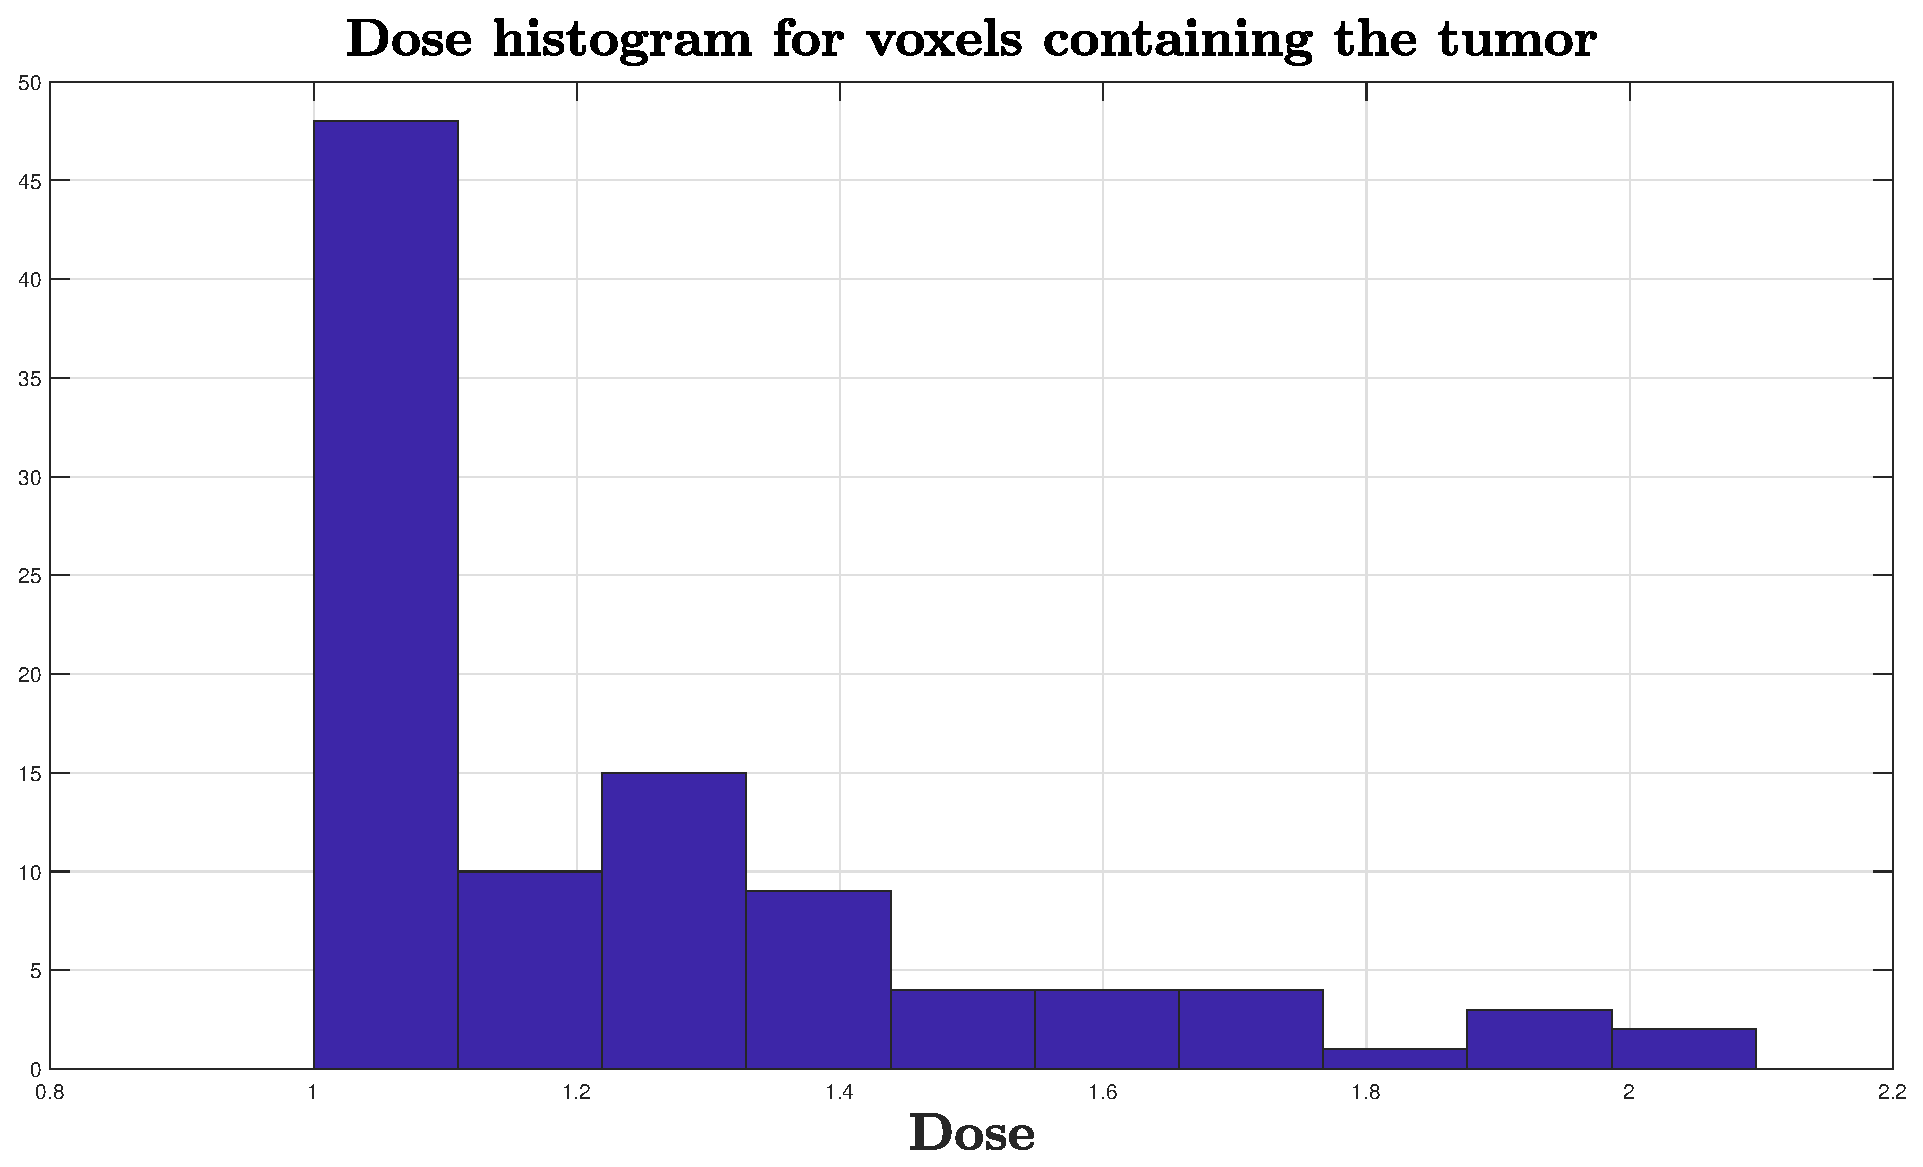
\includegraphics[scale=.45]{tumordose}
		\end{center}
	\end{figure}
	\begin{figure}[h!]
	\begin{center}
		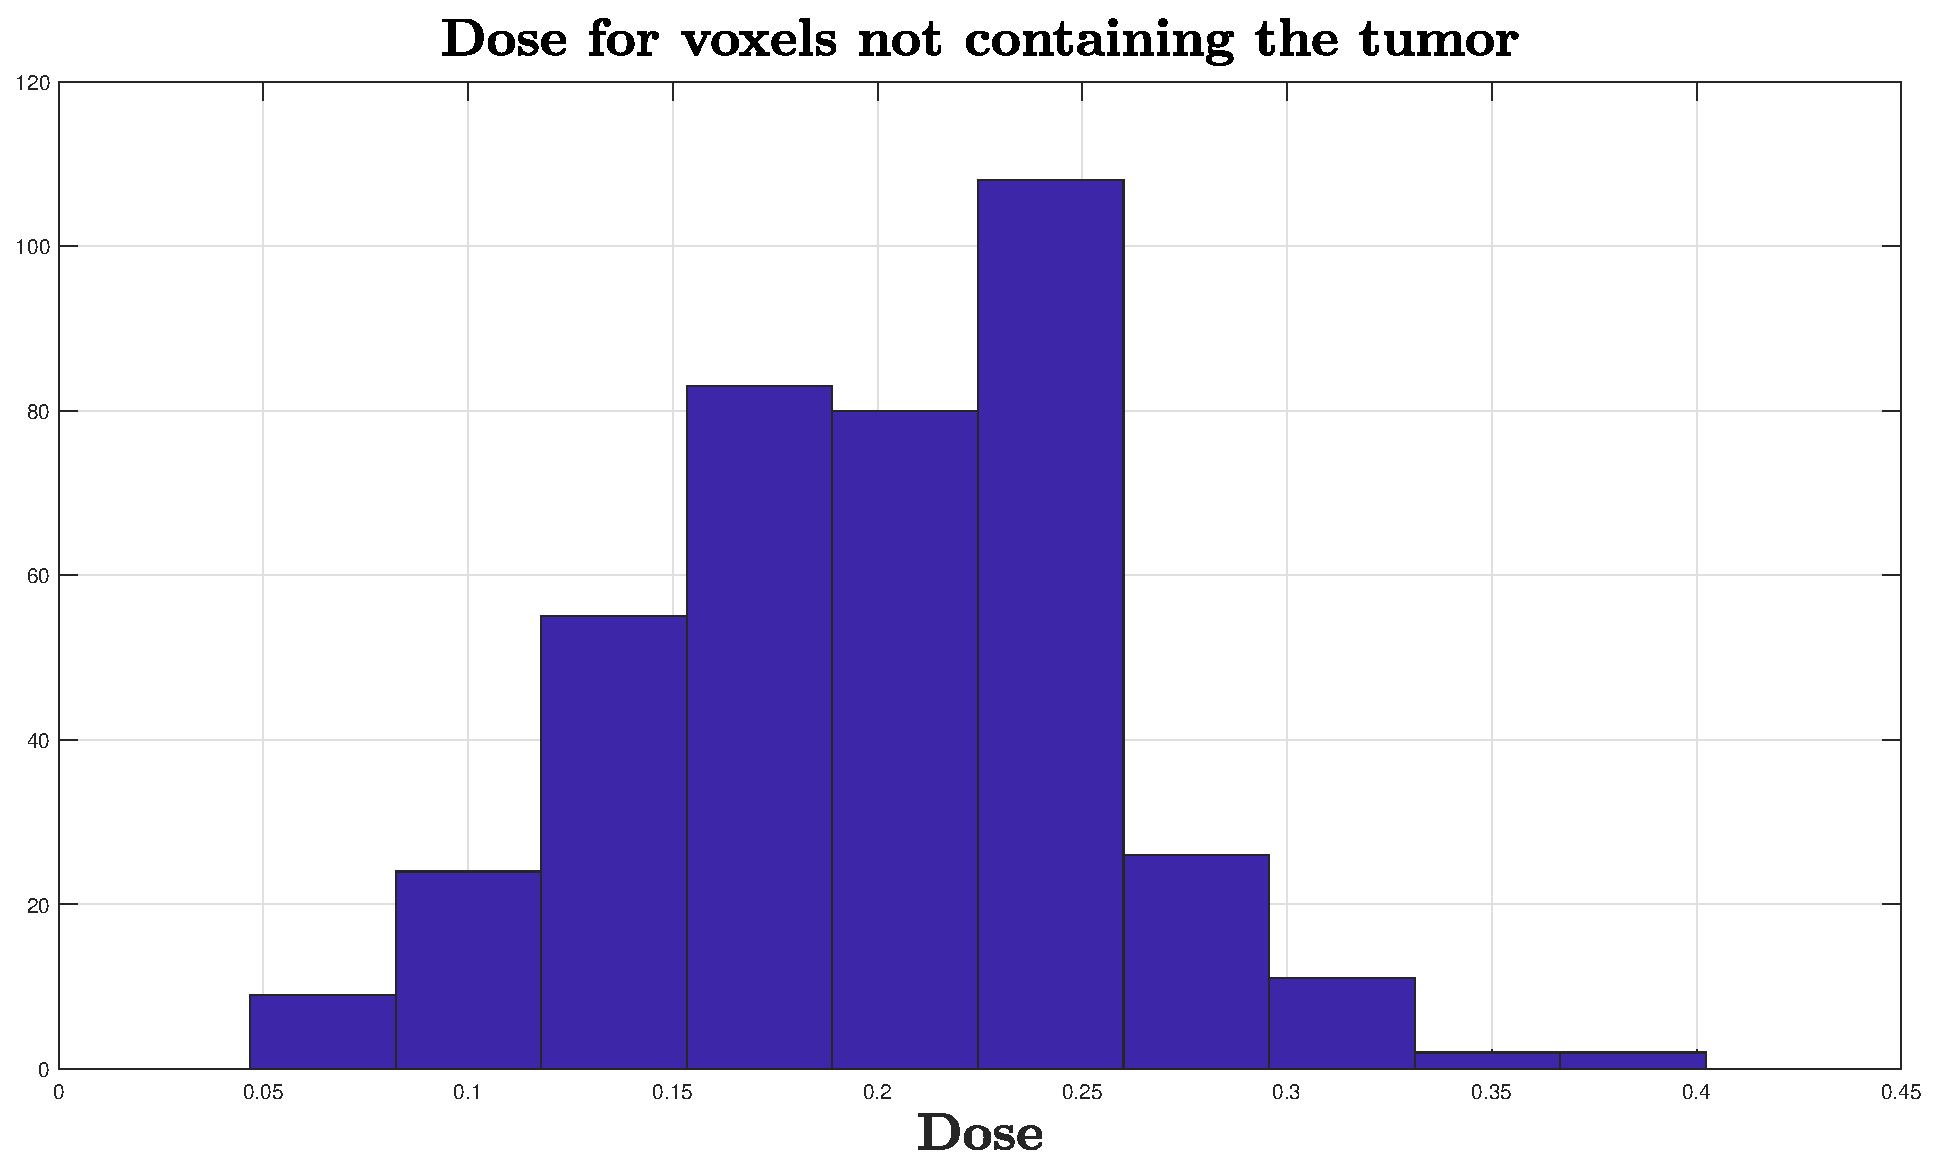
\includegraphics[scale=.45]{nontumordose}
	\end{center}
	\end{figure}	
	In the given dataset, voxels containing tumors require a minimum dose of 1, this condition has been met. It is also evident that a large number of voxels get the minimum dose. As expected, for voxels without the tumor, the condition that all their doses be less than $ D^{other} $ has not been met but a large portion of the data satisfy this condition.
\newpage
\section*{Code Appendix}
\subsection*{Problem 5}	
\lstinputlisting{Question_5.m}
\newpage
\subsection*{Problem 6}
\lstinputlisting{Question_6.m}
	
\end{Large}
\end{document}

